\documentclass[10pt,a4paper]{article}
\usepackage[utf8]{inputenc}
\usepackage[francais]{babel}
\usepackage[T1]{fontenc}
\usepackage{amsmath}
\usepackage{amsfonts}
\usepackage{amssymb}
\usepackage{listings}
\usepackage{pageGarde/HEIG_STY}
\usepackage[hidelinks]{hyperref}
\usepackage{lipsum}
\usepackage{fancyhdr} % En tetes / bas de page
\usepackage{siunitx} % needs texlive-science package on debian
\usepackage{tabularx}
\usepackage{pdfpages}
\newcommand{\tde}{Transfusion d'Éternité}
 
%marge des pages
\setlength{\textwidth}{16cm}
\setlength{\textheight}{24cm}
\setlength{\oddsidemargin}{0cm}
\setlength{\voffset}{-1.5cm}
\setlength{\headheight}{15pt}


\title{Projet de Gestion d'Entreprise}
\subtitle{\tde{}}
\author{João Miguel Domingues Pedrosa \\ Stephane Donnet \\ Loïc Haas \\ Nicolas Kobel}

\acro{GET}
\cours{Gestion d'Entreprise}
\date{\today}
\prof{Destine au Prof. Dider Gern}


\pagestyle{fancy}
%en-tête
\lhead{Groupe hypocras}
\chead{Rapport GET - Projet Hypocras}
\rhead{\theAcro}
 
%pied-de-page
\lfoot{HEIG-VD}
\cfoot{\today}
\rfoot{\thepage}

\begin{document}
\maketitle
\tableofcontents
\hspace{0.4cm}
\begin{figure}[h]
\centering

\includegraphics[width=0.3\textwidth]{../images/logo.png}
\end{figure}
\newpage
\section{Introduction}
Ce projet s'inscrit dans le cours de Gestion d'Entreprise donné aux étudiants de troisième année du departement TIC.
Dans ce projet nous mettons en oeuvre les techniques et connaissance acquise lors du semestre.

Le cadre de ce projet est une entreprise semi-fictive nommée \textit{\tde{}}.
Nicolas Kobel, avec une amie Mme Victory Jaques, est entrain d'étudier la création réelle de cette entreprise.
Les produits décrits ci-dessous sont des produits réels de cette entreprise, les chiffres présentés sont des extrapolations des premiers calculs financiers de Mme Jaques et M. Kobel.
Les autres informations ont étés crées pour ce rapport et n'ont pas (encore) étés réalisés.

Les auteurs aimeraient remercier Mme Jaques pour avoir accepter l'utilisation de son travail dans le cadre de ce projet.
\newpage
\section{L'entreprise}
\tde{} est une entreprise de création de boissons.
Elle produit de l'hypocras, une boisson alcolisée à base de vin et d'épices\footnote{\url{https://fr.wikipedia.org/wiki/Hypocras}}.

%\tde{} est une SàRL d'après le droit suisse avec siège à Lausanne.
Les deux fondateurs sont étudiants et s'investissent à titre personnel dans l'entreprise.
Ils travaillent à raison de 2 jours de 8 heures par mois chacun soit 32 heures de travail mensuelles.
L'entreprise ne compte pas d'autres employés.

Le produit est déstiné à la vente directe par internet ainsi qu'à la vente à des revendeurs (magasins et bars).
La répartition entre vente directe et vente au revendeurs est de 30/70.
\subsection{Le Produit}
\begin{figure}[h]
\centering
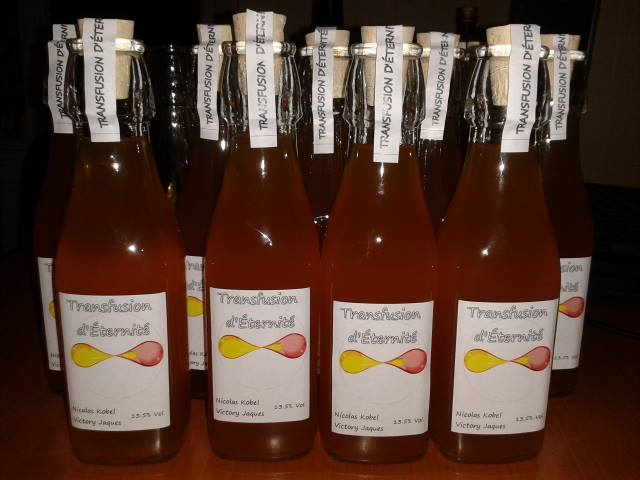
\includegraphics[width=0.5\textwidth]{../images/bouteilles.jpg}
\end{figure}

\tde{} propose pour le moment une gamme unique de produits, nommée \textit{Hypocras \tde{}}.
Il s'agit d'une boisson alcolisée à base de vin, miel et épices.

Le produit est décliné en deux variantes, blanc et rouge.
La seule difference est le vin utilisé comme base, les autres ingrédients et le processus de fabrication sont identiques.

La recette de fabrication s'inspire d'une recette d'hypocras antique conservée dans les écrits de Pline l'Ancien.
%Des variantes de cette recettes ont étés téstés par \tde{} et pouront servire comme base pour une gamme differente.
Le lien avec l'antiquité est pour \tde{} un signe de qualité et de durabilité qui sera éxploité dans les actions publicitaires.

\tde{} s'engage à présenter au client la meilleure qualité possible et propose un produit à base d'ingrédients si possible locaux et bio.
Ainsi le vin est fourni par des vignerons de la côte du lac léman cértifiés bio et le miel par des apiculteurs de la région de la gruyère.
Les épices réstantes sont elles aussi cértifiées de production biologique.

Le produit est présenté dans un packaging sobre et classique.
L'hypocras est vendue par bouteilles de 0.25l aux clients sur internet et aux magasins revendeurs.
La taille des bouteilles de revente pour les bars n'a pas encore étée fixée, mais se trouvera dans entre 0.5l et 1l.

Les bouteilles déstinées aux particuliers sont des bouteilles en verre carrés, refermées par un bouchon en liège.
Une étiquette contenant le nom et le logo de \tde{} ainsi que la teneur en alcool se trouve à l'avant de la bouteille.
Une étiquette avec les ingrédiants de base ainsi que leur provenance et des conseil de service se trouve au dos de la bouteille.

Les bouteilles vendues aux particuliers par biais du site internet sont accompagnés à l'envoi d'un feuillet explicant l'histoire de l'hypocras et de \tde{}.
% photo bouteille ici

%\lipsum
\subsection{Le Public Cible}
\tde{} cible un public romand, jeune et interéssé aux boissons "exotiques".
Par son côté médieval l'hypocras attire avant tout les passionnés d'histoire, de reconstitution et du fantastique.
Par conséquant les joueurs de rôle seront la principale cible du produit.

Ce public se retrouve régulièrement dans des conventions ou des événements participatifs, ainsi que sur des canaux de discussions en ligne, la rencontre avec les potentiels clients est facile à faire sur internet ou dans les dites conventions.
C'est aussi un public majoritairement jeune et donc habile avec les nouvelles technologies.
La vente par internet est donc une priorité.
\subsection{Préstations Supplémentaires}
En tant que préstation supplémentaire, \tde{} propose sur son site d'achat la possibilité de personnaliser le packaging.
Le client peut lors de la commande demander un carte avec un message personnalisé et l'envoi sous forme de paquet cadeau.
Cette carte au logo de l'entreprise est imprimé automatiquement dans les lieux de production, l'embalage se fait de manière manuelle.

Une autre possibilité est la commande sur le site avec possibilité de retrait de la marchandise chez un revendeur agréé.
En lieu d'un envoi matériel, le client à la possibilité d'imprimer un bon de retrait avec contrôle numérique éfféctué par le revendeur.
\section{Brevets}
\tde{} a breveté une machine permettant d'automatiser le processus de fabrication.
Il s'agit d'un mixeur/plaque chauffante avec divers compartiment qui ajoute à la base de vin les ingrédiants nécessaires à la production de l'hypocras.
Les pages suivantes contiennent le dépot du brevet.

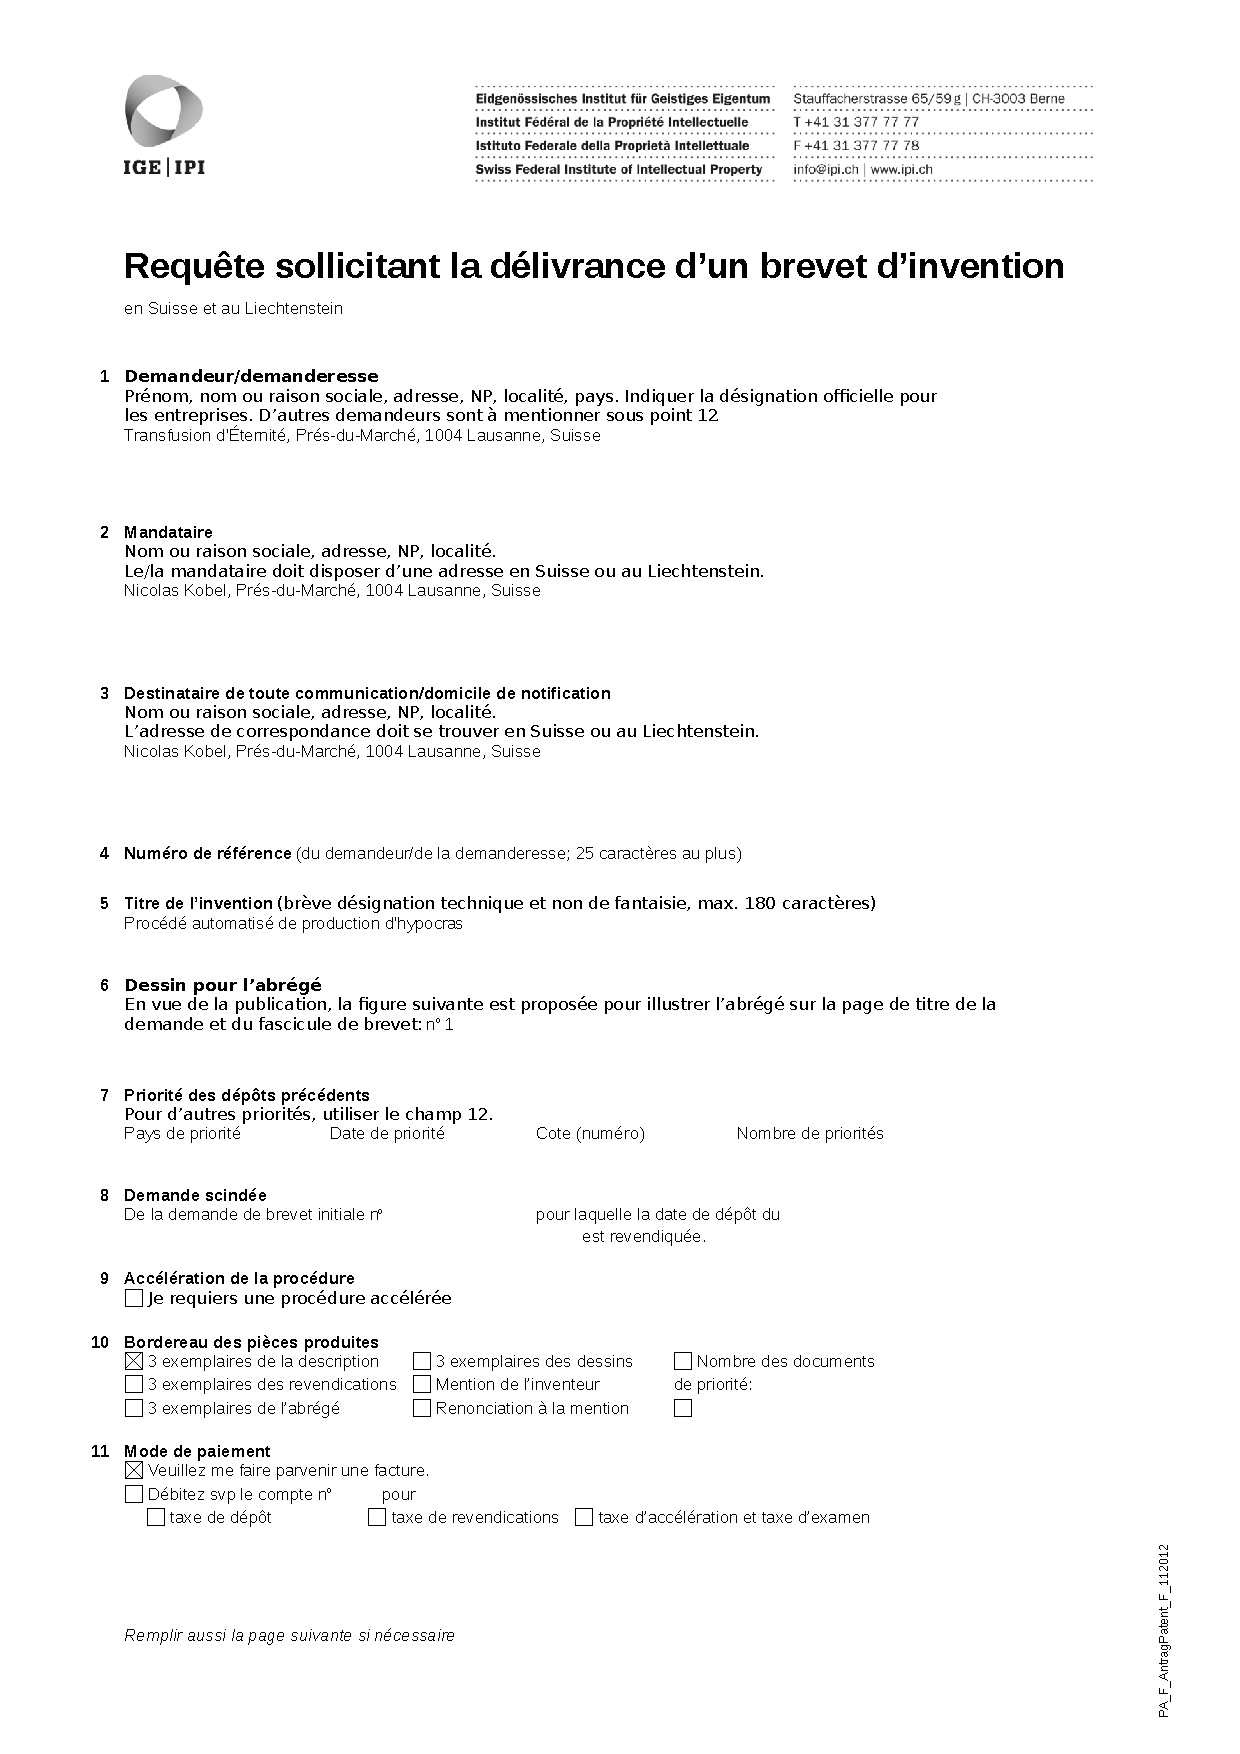
\includepdf[pages={1,2}]{../Annexe/requete_brevet.pdf}
\section{Dépot de Marque}
\tde{} est une marque enregistrée au sens du droit suisse.
La marque consiste en un nom et un logo déposé.
Les pages suivantes contiennent la demande de dépot de la marque.

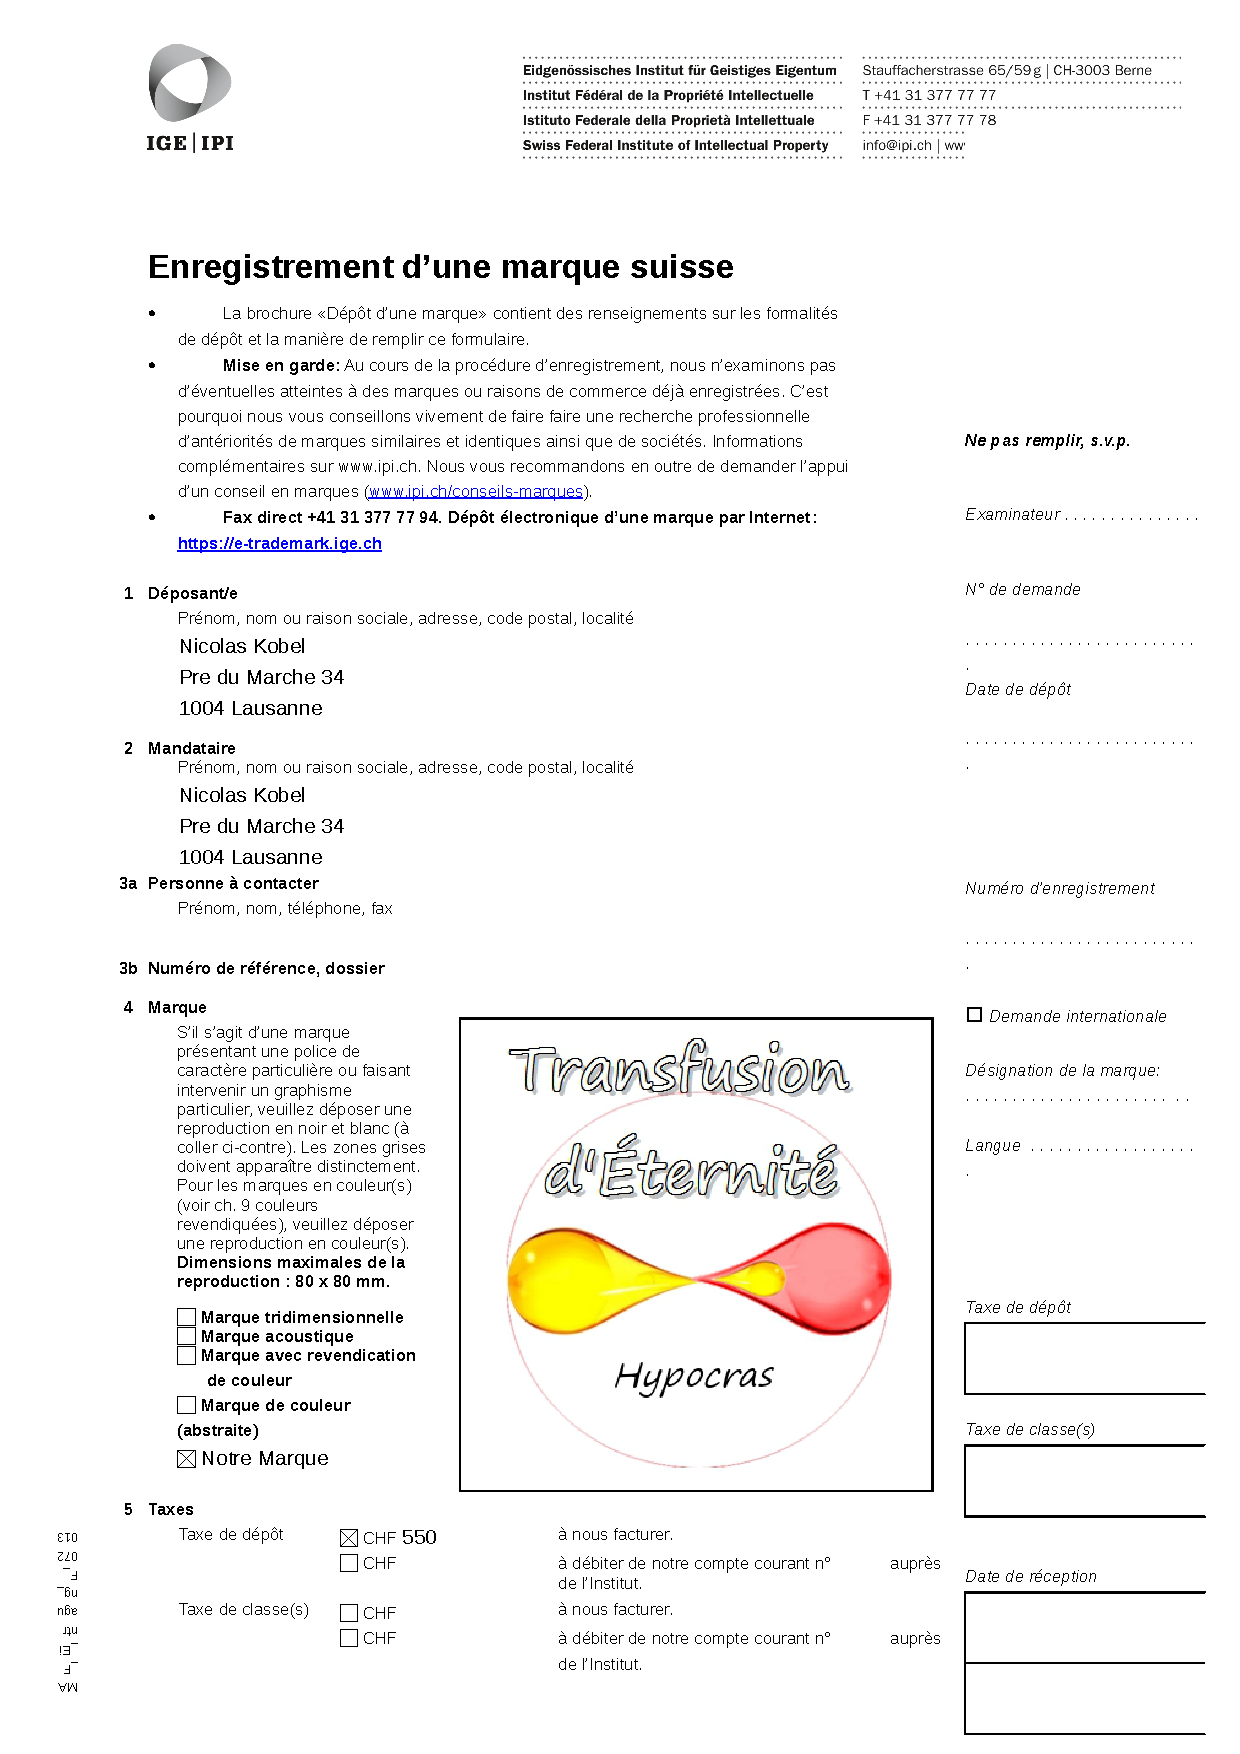
\includepdf[pages={1-3}]{../Annexe/depot.pdf}
\section{Processus}

\subsection{Fabrication}
Le processus de fabrication implique l'entreprise et le(s) fournisseur(s) de matières premières.
La fabrication est relativement simple, seule une période de maturation d'un mois doit être réspecté pour garantir la qualité du produit.
Cette pause rends la production sur commande impossible, \tde{} doit donc garantir posséder les stocks nécessaires à l'execution de sa mission.

Le processus est décrit en détails dans le graphe \ref{prod} ci-dessous.

\begin{figure}[h!]
\centering
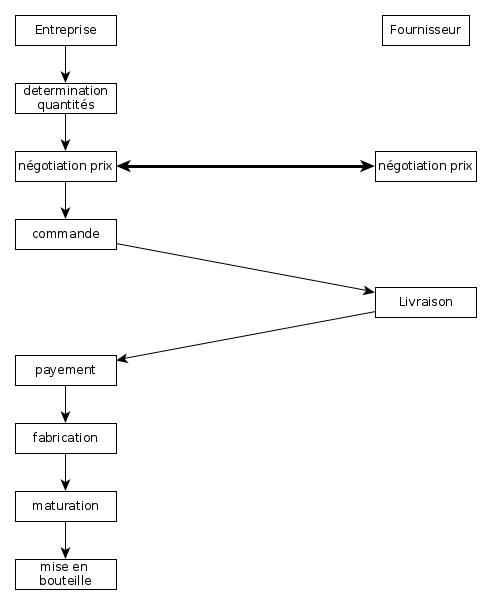
\includegraphics[width=0.5\textwidth]{../flowchart/prod.jpg}
\caption{Processus de fabrication}
\label{prod}
\end{figure}
\subsection{Vente Internet}
La vente par internet à été scindée en deux procéssus.
Le premier tel que détaillé dans le graphe \ref{cmdInternet} traite la commande au niveau du client.
Il a la possibilité de commander en plusieurs parties, si les stocks ne sont pas disponibles pour traiter la commande complète.

Le deuxième processus détaillé dans le graphe \ref{cmdUsine} concerne le traitement des commandes aux sein de l'entreprise.
Nous gérons içi aussi le cas de la commande devant être scindée.
Dû au temps de maturation du produit (environ 1 mois) il nous est impossible de produire à la commande.
Il est donc possible que dans un premier temps les prévisions de vente ne corréspondent pas à la demande.
Des statistiques menées au cours de l'activité permetterons d'ajuster la production.
\begin{figure}[h!]
\centering
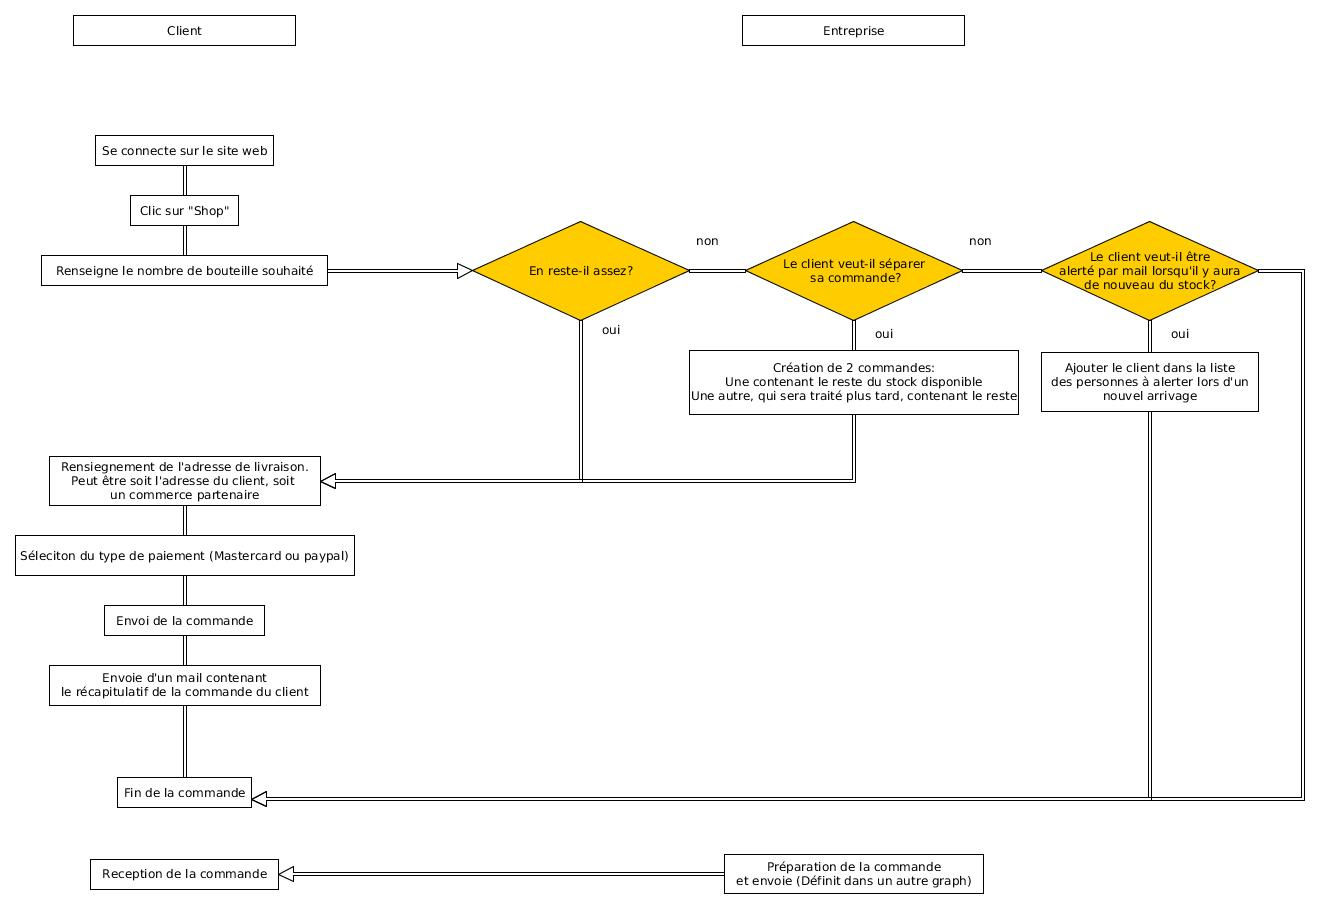
\includegraphics[width=0.9\textwidth]{../flowchart/commandeInternet.jpg}
\caption{Processus de traitement de commande, côté client}
\label{cmdInternet}
\end{figure}

\begin{figure}[h!]
\centering
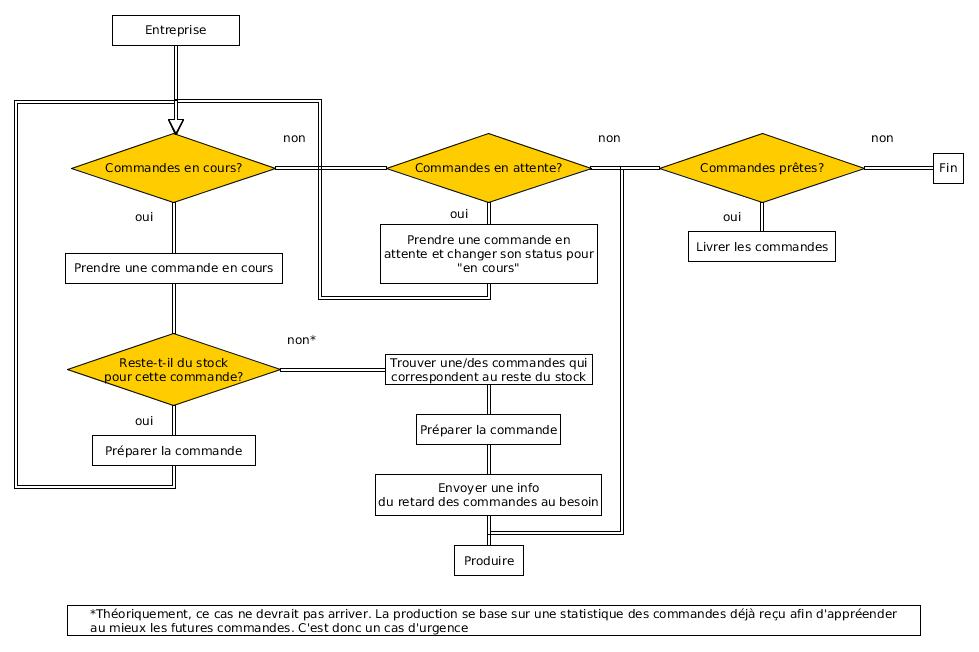
\includegraphics[width=0.9\textwidth]{../flowchart/commande.jpg}
\caption{Processus de traitement de commande, côté entreprise}
\label{cmdUsine}
\end{figure}
\clearpage
\subsection{Vente aux Redistributeurs}
La vente aux redistributeurs (processus \ref{redist}) est aussi relativement simple à gérer.
Nous demandons aux distributeurs des feed-backs sur la vente de nos produits, sur-tout si c'est la première vente qu'ils font pour nous.

\begin{figure}[h!]
\centering
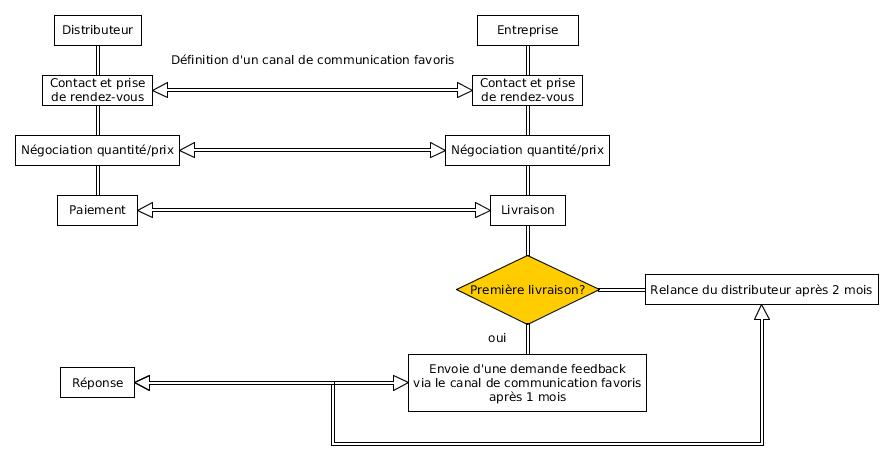
\includegraphics[width=0.9\textwidth]{../flowchart/distributeur.jpg}
\caption{Negotiations avec redistributeurs}
\label{redist}
\end{figure}

\clearpage
\section{Finances}
\tde{} table sur une production mensuelle moyenne de 100l d'hypocras.
Ce chiffre est le maximum réalisable par deux personnes et représente pour un produit de niche une bonne quantité de lancement.

C'est aussi, comme les calculs l'indiquent une quantité rentable.

Les calculs détaillés à pour chaque point ci-dessous se trouvent en annèxe.

\subsection{Prix de Fabrication}
Le prix de fabrication par litre d'hypocras comprends les matières premières, les produits pour le packaging, les frais d'envois et d'acheminement ainsi que les consommables nécessaires au filtrage.
Ils sont répartis ainsi :

\vspace{0.5cm}
\begin{tabular}{|l|S[table-format=4.2]|S[table-format=4.2]|}
\hline
& \textbf{Pour 1 L} & \textbf{Pour 100 L} \\\hline
Matières premières & 16.65 & 1665.00\\ 
Packaging & 9.60 & 960.00\\ 
Envoi et Acheminement & 2.50 & 250.00 \\
Consommables & 0.40 & 40.00\\\hline
\textbf{Total} & 29.15 & 2915.00\\\hline
\end{tabular}


\subsection{Depenses Fixes}
Les depenses fixes sont dûs à la location des lieux, les frais administratifs, l'amortissement des installations nécessaires à la production et aux salaires.

\vspace{0.5cm}
\begin{tabular}{|l|S[table-format=3.2]|S[table-format=3.2]|}
\hline
& \textbf{Coût Mensuel} & \textbf{Coût Annuel} \\\hline
Location & 2100.00 & 31200.00\\
Frais Admin & 500.00 & 6000.00 \\
Ammortissements & 104.16 & 1250.00\\
Salaires & 640.00 & 7680.00 \\\hline
\textbf{Total} & 3344.16 & 46130.00 \\\hline
\end{tabular}

\subsection{Objectifs Commerciaux}
L'entreprise étant un projet annexe \tde{} ne cherche pas d'énormes profits.
Un gain ésperé mensuell net de \textbf{CHF 500.00} permet à \tde{} de se remettre de mois moins favorables.
\subsection{Prix du Produit}
Le produit étant présenté comme un produit de luxe le prix le reflete.
Les fournisseurs, qui se font une marge sur le produit et pour qui nous n'avons peu de frais d'acheminements obtiendron la bouteille à un prix de \textbf{CHF 14.50}.

Les clients du site web devronts s'aquitter du prix d'envoi (inclus dans le prix de vente) ainsi que d'une majoration pour la charge administrative supplémentaire.
La boutielle leur est donc proposée à \textbf{CHF 21.50}.
\subsection{Rentabilité}
Sur une base de 100L d'hypocras produite et vendue par mois nous avons le calcul suivant :

\vspace{0.5cm}
\begin{tabular}{|l|S[table-format=3.2]|S[table-format=3.2]|}
\hline
& \textbf{Dépenses} & \textbf{Entrées} \\\hline
Frais de production & 2915.00 & \\
Frais Fixes & 3344.16 & \\
Vente Internet & & 2580.00 \\
Vente aux Distributeurs & & 4060.00 \\\hline
\textbf{Total} & 6259.16 & 6640.00 \\\hline
\end{tabular}

\vspace{0.5cm}
L'entreprise fait dans ces conditions un bénéfice de \textbf{CHF 380.84}.
L'exercice est rentable, mais l'objectif fixé de CHF 500.00 n'est pas atteint.
Pour l'atteindre \tde{} devrait augmenter sa production mensuelle, ce qui n'est pour le moment pas envisageable.
\subsection{Plan de Trésorerie}
Le plan de trésorerie ci-dessous présente les entrées et sorties pour l'année de lancement.
Nous supposons que les revendeurs payent à livraison du produit.
Il ne sera pas possible pour le client de payer sur facture, \tde{} n'acceptant uniquement les payements en avance.
Ainsi nous nous epargnons les soucis des factures réstées impayées.

Le capital de d'investissement est fourni à part égale par les deux fondateurs et comporte CHF 6000.00.
Les fondateurs sont remboursés par les bénéfices de l'entreprise.

Afin de pouvoir investir dans les CHF 1300.00 d'achats immobilisant (matériel pour la production), un pret de CHF 1700.00 doit être demandé.
Ce prêt peut se faire à très court terme, les calcules indiquent qu'en septembre les surplus de trésorerie auront dépassés ce montant.

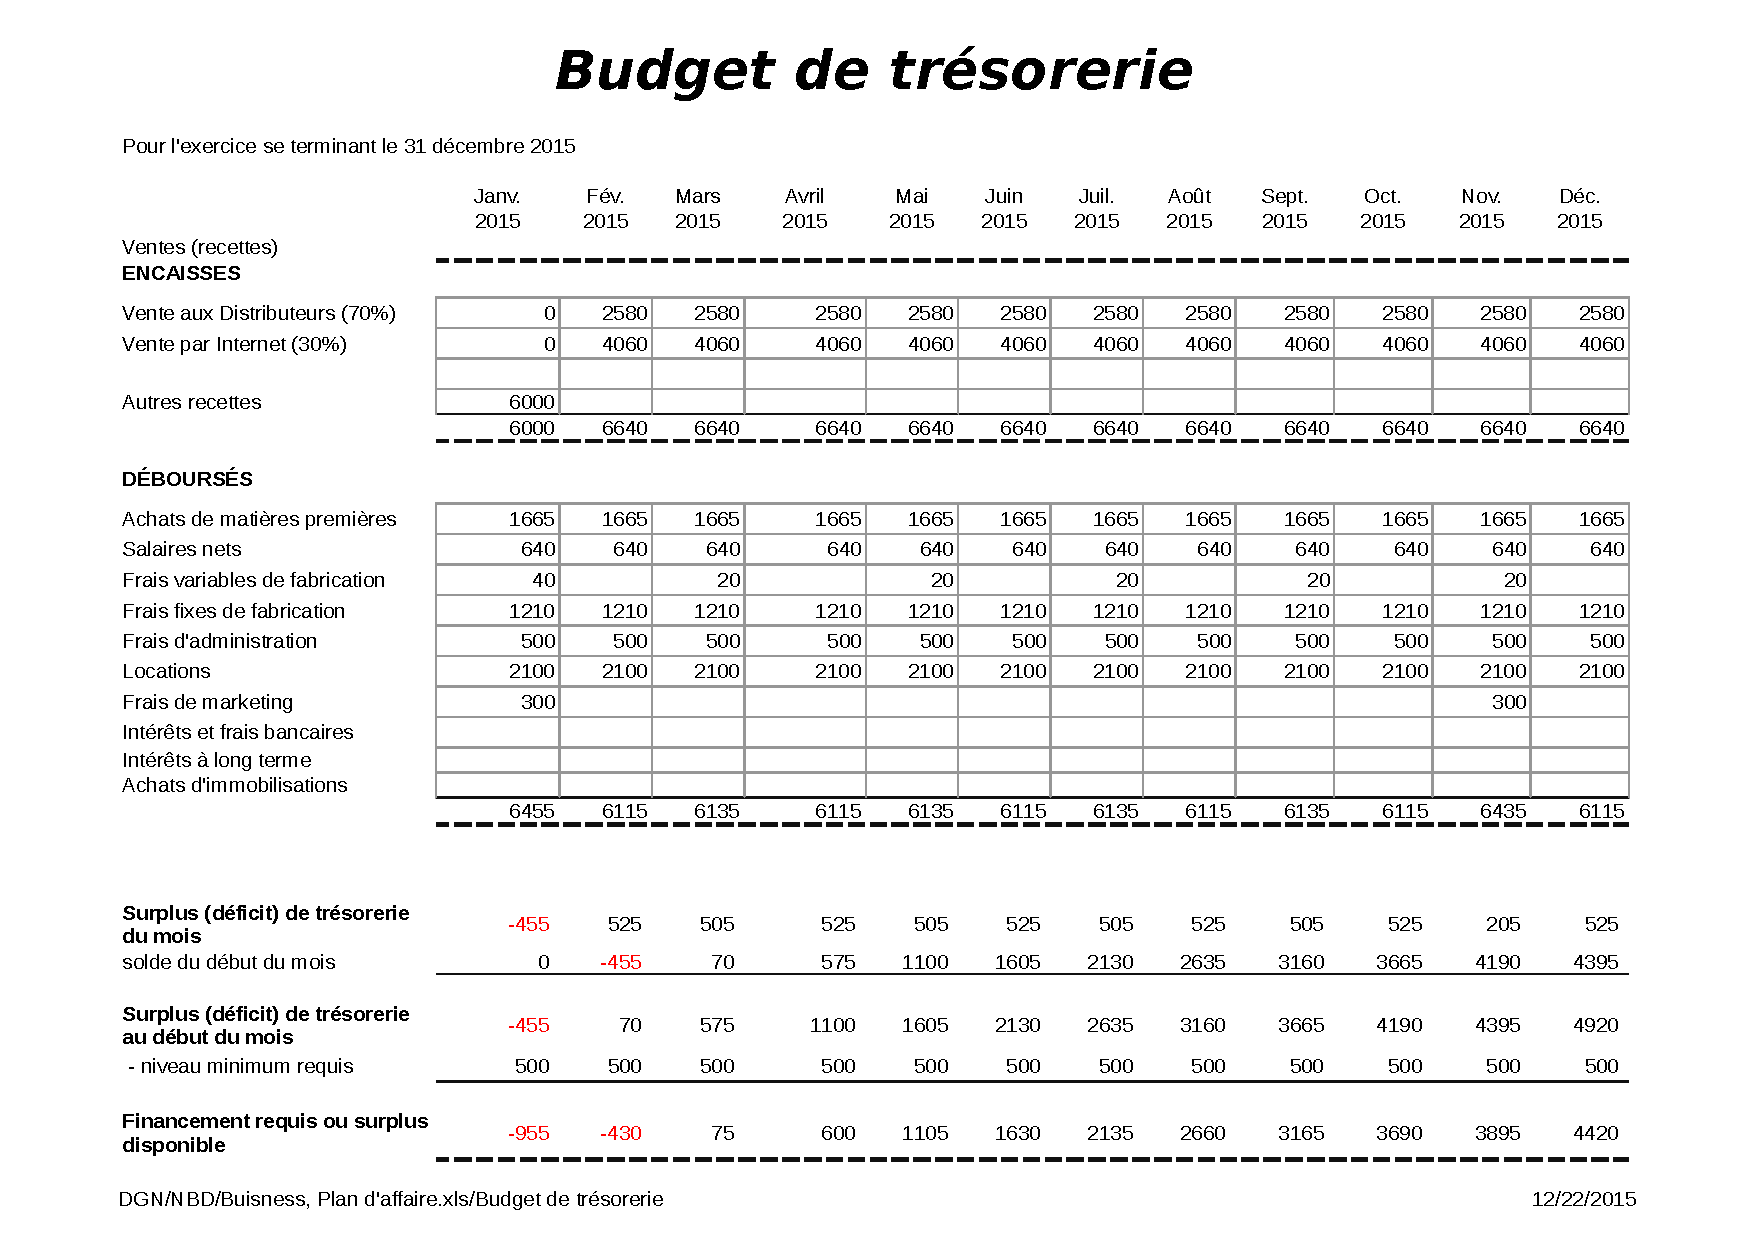
\includepdf[landscape]{../Annexe/tresor.pdf}
\section{Actions Publicitaires}
Les actions publicitaires envisagées sont orienté vers la rencontre directe avec nôtre public cible.

Dans ce cadre nous présenterons nos produits lors de conventions de jeux de rôles ainsi que lors de reconstitutions historiques.
Lors de ces présentations nous propseront des dégustations et de la vente directe.
Il est aussi envisageable de faire des démonstrations intléractive du brassage lors de conventions de durée moyenne à longue.

Nous souhaitons aussi rechercher un public plus large, par le biais de dégustations chez des réstaurateurs proposant une grande variété de boissons artisanales.

La campagne de lancement se fera dans la région ciblée, à savoir la suisse romande.
Dans un premier temps des distributions de flyers et de l'affichage se feront à Lausanne.
Une campagne similaire est envisagée dans les autres villes romandes.

La période de noël est vue par \tde{} comme une des deux periodes à forte demande (l'autre étant celle des conventions de jeux de rôles en été).
A cette occasion nous éspèrons atteindre un maximum de clients potentiel avec une grand présence lors des marchés de noël.
Les clients connus receverons lors de cette période des promotions afin de les fidéliser.
\section{Annexes}
\subsection{Details Matières Premières}
\begin{tabular}{|l|S[table-format=4.2]|S[table-format=4.2]|}
\hline
& \textbf{Pour 1 L} & \textbf{Pour 100 L} \\\hline
Vins (80 cl/80 l) & 8.50 & 850.00 \\
Miel (330g / 33 kg) & 5.60 & 560.00 \\
Epices & 2.61 & 261.00 \\\hline
\textbf{Total} & 16.71 & 1671.00\\\hline
\end{tabular}
\subsection{Details Packaging}
\begin{tabular}{|l|S[table-format=4.2]|S[table-format=4.2]|}
\hline
& \textbf{Pour 4 bouteilles (1 L)} & \textbf{Pour 400 bouteilles (100 L)} \\\hline
Bouteilles & 6.00 & 600.00 \\
Bouchons Lièges & 1.20 & 120.00 \\
Etiquettes (impression comprise)& 2.41& 241.00 \\\hline
\textbf{Total} & 9.61 & 961.00\\\hline
\end{tabular}



\end{document}